\section{Muon Background}

Over the course of the last several years the frequency and supernova significance, $\xi$, of false supernova alerts has risen, see Figure~\ref{fig:SNDAQtriggershisto}. In \cite{vbaumaster} it has been shown that atmospheric muons are main cause of false triggers and are correlated to the muon hit rate, see Figure~\ref{fig:muratetriggersig}. The nature of these muons beyond the number of DOMs they trigger however was not explored. The rising significance of the alerts was initially attributed to increasing solar activity as the sun approached the maximum of the 11-year solar cycle, see Figure~\ref{fig:solarcycle}, as the temperature of the upper atmosphere rises with increasing solar irradiation. The rise in the significances should not be significantly effected by these long-term effects to the flux or energy spectrum of the atmospheric muons, as the background region is defined over significantly shorter timespan than these effects. The question remains whether there are distinct features in these events that can be extracted from the information provided by the DAQ. 

\begin{figure}[h]
  \begin{center}
    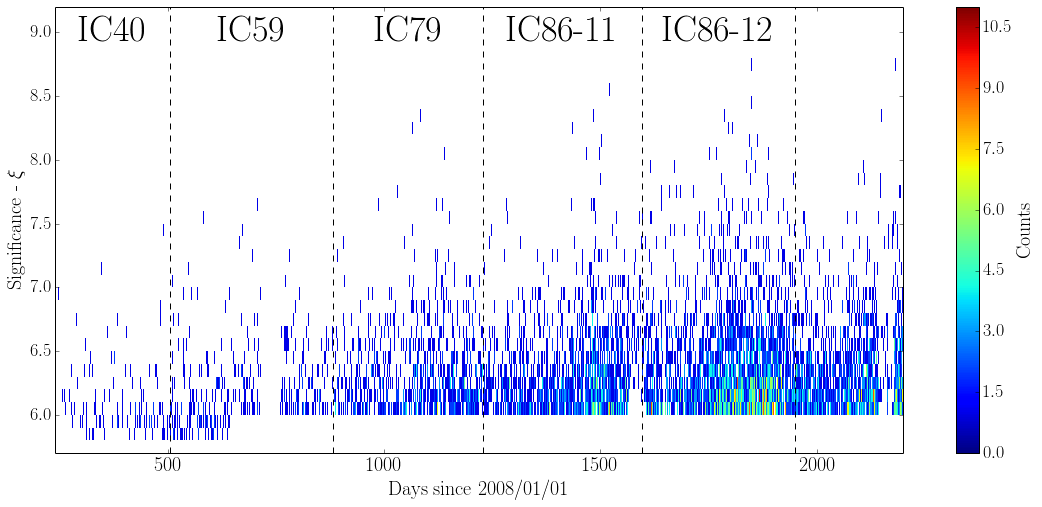
\includegraphics[width=1\textwidth]{./figures/IC40IC863AlertsSigmavsTwebsiteparser.png}
  \end{center}
  \caption{SNDAQ significances, $\xi$, over threshold (6) from IC40 to present. \label{fig:SNDAQtriggershisto}}   
\end{figure}

% \begin{figure}[h]
%   \begin{center}
%     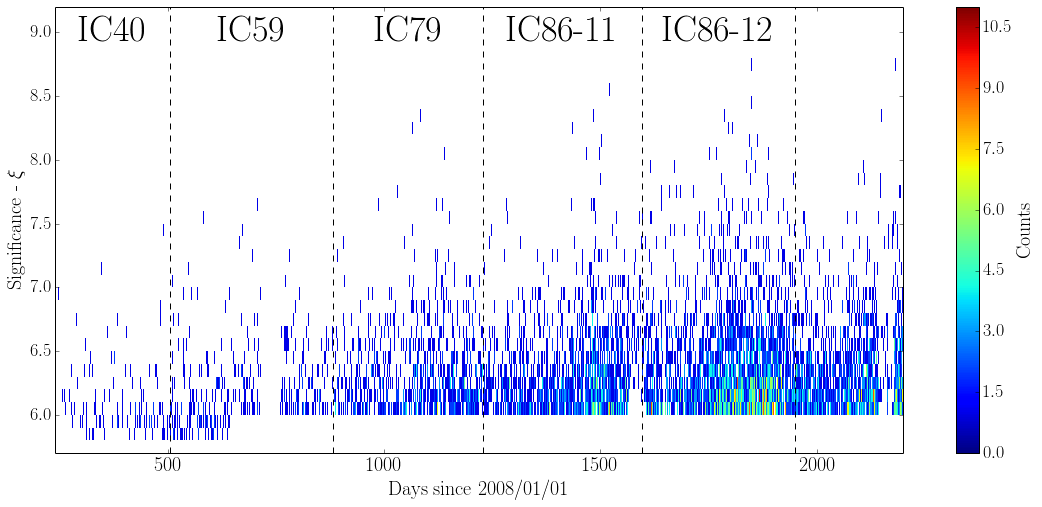
\includegraphics[width=1\textwidth]{./figures/IC40IC863AlertsSigmavsTwebsiteparser.png}
%   \end{center}
%   \caption{SNDAQ significances, $\xi$, over threshold (6) from IC40 to present. \label{fig:muratetriggersig}}   
% \end{figure

% \begin{figure}[h]
%   \begin{center}
%     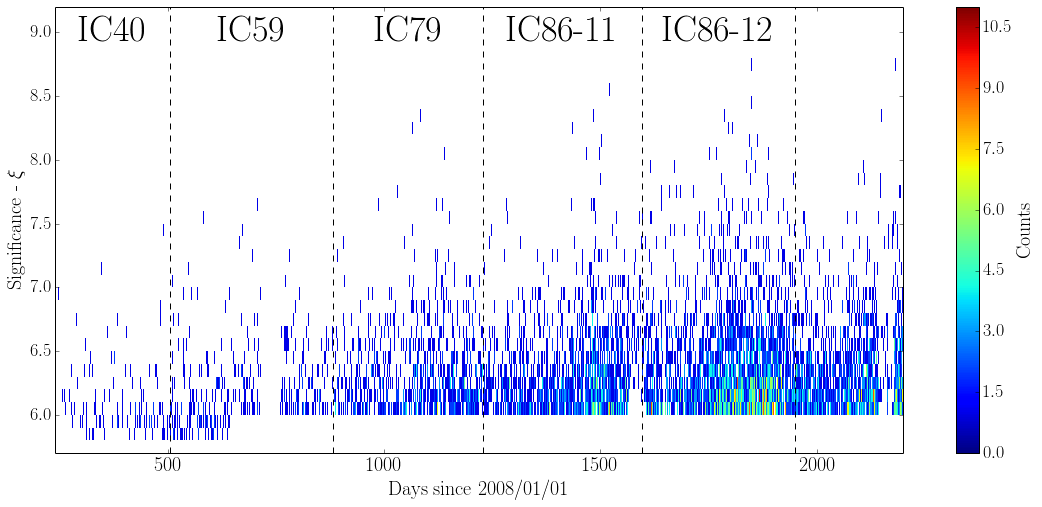
\includegraphics[width=1\textwidth]{./figures/IC40IC863AlertsSigmavsTwebsiteparser.png}
%   \end{center}
%   \caption{SNDAQ significances, $\xi$, over threshold (6) from IC40 to present. \label{fig:solarcycle}}   
% \end{figure}

In \cite{vbaumaster} the Data Storage and Transmission (DST) data was used determine the muon hit rate from the SMT8 trigger rate and the number of DOMs that were triggered, ``nchannel'' (nchan), of the triggers. This muon hit rate is shown to be correlated to the $\xi$ as determined by the the supernova online analysis. There was however no consideration for other triggers, such as the \emph{String Trigger} and the \emph{Volume Trigger}. These triggers could help identify large muon events that cause false supernova triggers more readily. For this reason, a study of the correlation of trigger rates for SMT8, SMT3, Volume Trigger, and String Trigger with supernova false trigger will be performed. For the supernova false triggers with $\xi > 6$, the trigger rate for all triggers of interest will be determined from the Super Data Storage Tape (sDST). The sDST data contains all individual triggers and time stamps thereof. The DST data only contains a bitmask that accounts for the the presence of a trigger, but not a count. This will help in account for possible overlapping triggers and give a better picture of the timing distribution. In order to ensure proper comparison of the data, the same rolling window as used in the SNDAQ online analysis is applied to the sDST data. The data is than split into the background and signal region and comparison of the trigger rates, nchannel distributions, and direction of events will be performed.

Investigating other triggers will remove some of the shortcomings of the analysis in \cite{vbaumaster}:

\begin{itemize}
  \item SMT8 rate of DST data does not reflect the real SMT8 rate
  \item SMT8 trigger does not consider any geometry information beyond the local coincidence (LC) condition
  \item Supernova scalers have a lower energy cutoff than SMT8, i.e. is SMT8 the best possible measure or is there a different trigger?
\end{itemize}

The DST does not contain all the trigger information, as overlapping triggers are compressed into a bitmask that only accounts for the the presence of a trigger, but not a count. SMT8 triggers can overlap because of their extended readout windows as required by the EventBuilder. The probability of overlap of two SMT8, assuming \unit[2100]{Hz} trigger rate for SMT8 and a \unit[10]{$\mu$s} readout overlap window, is $\approx$ 0.2\%. This should have an minuscule effect on the correlation method. When looking at all possible triggers the overlap between different triggers approaches 1. Additional other triggers, mainly the \emph{Volume Trigger}, have a much higher rate ($\approx \unit[3300]{Hz}$), which leads to a much higher possibility of overlap for these triggers. 

The SMT8 trigger does not consider the geometry of the events and the detector beyond the geometry requirement of the local coincidence (LC) condition. The geometry and time span of a muon event are completely different than that for a supernova event. Individual muon events would only illuminate certain areas of the detector for $\mathcal{O}$(\unit[1 - 10]{$\mu$s}), while the supernova event illuminates the entirety of the detector over the course of $\mathcal{O}$(\unit[1 - 10]{s}). Looking at triggers that do have stricter geometric constrains may help identifying muon events. Also the \emph{Volume Trigger}'s much higher rate may yield more information about lower energy muons that the supernova scalers are sensitive to, but not SMT8. 

In addition to the trigger rate aspect. The comparison of nchan distribution and the location of the ``center-of-gravity'', where most of the hits are clustered, of the events between the signal region and the background region will be performed. 


  % \item Sensitivity of SMT8 trigger to supernova signals was never established
